%%%%%%%%%%%%%%%%%%%%%%%%%%%%%%%%%%%%%%%%%%%%%%%%%%%%%%%%%%%%%%%%%%%%%%
%% manuscript.tex
%% Decoupling smoothness, accuracy, and kinematic invariance in
%% biological reach: an ablation study of an equilibrium-point
%% controller in a 34-muscle arm model
%%
%% Target venue : Biological Cybernetics (Springer)
%% Source       : paper/manuscript.md (Markdown master) --- converted via
%%                pandoc + manual cleanup. The Markdown remains the
%%                authoritative draft until journal acceptance.
%% Status       : Compile-ready MVP (2026-05-06).
%%                In-text citations are still in plain-text form
%%                "(Author year)"; conversion to natbib \citet/\citep
%%                with a separate references.bib is a follow-up step.
%%%%%%%%%%%%%%%%%%%%%%%%%%%%%%%%%%%%%%%%%%%%%%%%%%%%%%%%%%%%%%%%%%%%%%

%% Bio Cyb uses Springer Basic (SPBASIC) name-year style.
\documentclass[sn-basic]{sn-jnl}

%% sn-jnl.cls (this 2019 mirror) calls \SetFootnoteHook and
%% \DeclareNewFootnote inside \AtBeginDocument without loading the
%% package they come from. Load manyfoot here so those commands resolve.
\usepackage{manyfoot}

%% Standard packages
\usepackage{graphicx}
\usepackage{amsmath,amssymb,amsfonts}
\usepackage{amsthm}
\usepackage{booktabs}
\usepackage{multirow}
\usepackage{xcolor}
\usepackage{textcomp}
\usepackage{geometry}
\usepackage{hyperref}

%% Pandoc converts markdown lists with \tightlist; provide a no-op so the
%% .tex compiles even if Pandoc's emit changes.
\providecommand{\tightlist}{\setlength{\itemsep}{0pt}\setlength{\parskip}{0pt}}

\raggedbottom

\begin{document}

\title[Decoupling kinematic invariance in biological reach]{Decoupling smoothness, accuracy, and kinematic invariance in biological reach: an ablation study of an equilibrium-point controller in a 34-muscle arm model}

\author*[1]{\fnm{Jun} \sur{Kobayashi}}\email{kobayashi.jun184@m.kyutech.ac.jp}

\affil*[1]{\orgdiv{Department of Intelligent and Control Systems, Graduate School of Computer Science and Systems Engineering}, \orgname{Kyushu Institute of Technology}, \orgaddress{\street{680-4 Kawazu}, \city{Iizuka}, \state{Fukuoka}, \postcode{820-8502}, \country{Japan}}}

\abstract{Engineering controllers solve musculoskeletal reaching but typically violate the kinematic invariants of human reach: bell-shaped speed profiles, near-straight paths, and a peak-velocity time at 40--50\,\% of movement duration. For the MyoSuite myoArm (20-DoF, 34 Hill-type muscles) we implement a biologically motivated controller combining (i) Feldman's $\lambda$-equilibrium-point hypothesis, (ii) a minimum-jerk virtual trajectory $\boldsymbol{\lambda}(t)$, (iii) a 200~ms visuomotor correction, and (iv) $\gamma$-compatible spinal reflexes (Ia, Ib, reciprocal inhibition). Across $n=50$ randomised targets the full controller is practically equivalent in accuracy to an \textbf{endpoint-PD~+~spinal} baseline (Cohen's $d=+0.03$ on minimum tip error of $\approx 100$\,mm, within a pre-defined $\pm 20$\,mm equivalence margin) while halving peak speed ($1.78$ vs $3.90$\,m\,s$^{-1}$, $d=-7.39$) and reducing jerk by 40\,\% ($d=-1.74$). Only the variant with stretch reflexes brings the velocity-peak ratio into the canonical human range ($0.40$--$0.50$). Straightness remains below the human reference, so we frame the result as a \textit{partial} reproduction of the bell-shape and smoothness invariants, not full human-like reach. A factorial ablation ($n=20$) attributes separable kinematic axes to distinct biological control layers: the virtual trajectory primarily controls smoothness, visuomotor feedback primarily controls accuracy, and reflexes primarily control velocity-peak timing. An attempted online cerebellar correction in joint or $\lambda$ space did not improve performance, consistent with the cerebellum acting as a slow inverse-model learner rather than a within-trial steerer. The result is mechanistic rather than task-optimal.}

\keywords{equilibrium-point hypothesis, virtual trajectory, visuomotor feedback, spinal reflexes, musculoskeletal model, ablation study}

\maketitle

\section{Introduction}

\subsection{Biological reach has structured invariants that
engineering controllers tend to
violate}

Human upper-limb reach exhibits a small set of kinematic regularities
that hold across speeds, distances, postures, and even loaded
conditions. End-effector speed follows an approximately bell-shaped
profile whose peak occurs at 40--50 \% of movement duration \citep{morasso1981, flashhogan1985}; the hand path between two points is nearly
straight in extrinsic space; and the time-derivative of acceleration
(jerk) is minimised in the sense of \citet{hogan1984}. These properties are
maintained even when the underlying joint trajectories are highly
non-linear, suggesting that the central nervous system plans in a
representation in which they are natural constraints rather than
emergent costs.

Modern musculoskeletal benchmarks such as MyoSuite \citep{caggiano2022} make it possible to simulate a 34-muscle Hill-type arm and to test
motor-control hypotheses in a setting that retains realistic muscle
dynamics. The default control schemes available in this setting ---
proportional--derivative (PD) endpoint controllers, model predictive
control, and reinforcement-learning policies --- typically solve the
task but produce motion that visibly violates the human invariants: high
initial peak speeds (\(3\)--\(4\) m s\(^{-1}\)), early peak-velocity
times (often within 5--10 \% of movement duration), and oscillatory
residuals near the target. The question we address in this paper is
whether a controller that is itself built from biological control
hypotheses can match the engineering baseline on accuracy \emph{while}
reproducing the canonical invariants, and if so, which component is
responsible for each invariant.

\subsection{Theoretical framework: $\lambda$-EP, virtual trajectory, and
visuomotor
feedback}

Three mature ideas in motor neuroscience together suggest a complete
controller. \textbf{Feldman's $\lambda$-equilibrium-point hypothesis} \citep{feldman1966, feldman1986, bizzi1976} posits that the descending command
specifies, for each muscle \(i\), a length threshold \(\lambda_i\) above
which the muscle is recruited. Activation is generated locally by
\(a_i = \mathrm{clip}(c\cdot\max(L_i - \lambda_i, 0),\,0,\,1)\) where
\(L_i\) is the current actuator length; the limb settles into the
equilibrium that balances the resulting muscle forces and external
loads, with no need for the brain to invert the dynamics. The
\textbf{virtual-trajectory} extension \citep{feldmanlevin1995, latash1993} replaces the static \(\boldsymbol{\lambda}_{\rm target}\) with a
smooth time-varying trajectory \(\boldsymbol{\lambda}(t)\) --- for
example, a minimum-jerk interpolation --- between the initial threshold
vector and the target one. Finally, \textbf{online visuomotor feedback}
\citep{saundersknill2003, sarlegnasainburg2009} provides a slow ($\approx$
100-- 200 ms latency) correction in which the central nervous system
re-estimates the target threshold from the observed tip position; the
error in \(\boldsymbol{\lambda}_{\rm target}\) is corrected without
disrupting the ongoing virtual trajectory. Embedded within the spinal
cord, \textbf{$\gamma$-compatible stretch reflexes} \citep{prochazka1989, loeb1984}, Golgi-tendon load feedback, and reciprocal inhibition shape the
activation locally on a 20--30 ms timescale and prevent co-contraction.
We retain the architectural slot for descending $\gamma$-motoneuron modulation
\citep{prochazka1989} but disable it in our production controller, since
pilot experiments showed no benefit on the metrics of interest (§3,
ablation).

These ideas have been tested individually in low-dimensional models or
in single-joint preparations. To our knowledge, they have not been
combined and ablated factorially in a high-dimensional Hill-type
musculoskeletal arm against an engineering baseline.

\subsection{Contributions}

We make four contributions.

\begin{enumerate}
\def\labelenumi{\arabic{enumi}.}
\tightlist
\item
  We implement a full biological reach controller for MyoSuite that
  simultaneously incorporates the $\lambda$-EP hypothesis, a minimum-jerk
  virtual trajectory, a periodic visuomotor correction, and a stack of
  spinal reflexes (Fig.~\ref{fig:5}). The implementation is MIT-licensed and is
  archived as \href{https://doi.org/10.5281/zenodo.19948021}{Zenodo
  \texttt{10.5281/zenodo.19948021}} (GitHub mirror:
  \href{https://github.com/jkoba0512/myoarm-lambda-ep}{\texttt{jkoba0512/myoarm-lambda-ep}}),
  with reproduction commands documented in the repository README.
\item
  We show that this controller is practically equivalent to an
  \textbf{endpoint-PD + spinal} baseline --- a Cartesian PD descending
  command sharing the same spinal reflex layer (§2.6) --- on minimum tip
  error (\(n = 50\), Cohen's \(d = +0.03\); only a small \(\approx 10\)
  mm paired residual, within a pre-defined \(\pm 20\) mm equivalence
  margin) while halving peak speed, reducing jerk by 40 \%, and bringing
  the velocity-peak ratio into the canonical human range (Fig.~\ref{fig:1}).
  End-effector paths are also straighter than the engineering baseline
  (Fig.~\ref{fig:3}), although both controllers fall short of the human
  straightness reference and the absolute residual error remains
  \(\approx 100\) mm; we therefore frame this as a partial --- not a
  full --- reproduction of human reach kinematics.
\item
  We perform a factorial ablation (\(n = 20\) per condition) of the
  three biological components and report a structured decomposition of
  their effects (Fig.~\ref{fig:4}): the virtual trajectory dominates the
  smoothness axis, visuomotor feedback dominates the accuracy axis, and
  stretch reflexes dominate the velocity-peak-timing axis. We make the
  contribution structure explicit by reporting both the primary
  (block-diagonal) and the secondary effects, the latter including a
  constructive contribution of the virtual trajectory to peak timing and
  a moderate cost of reflexes on peak-speed regulation.
\item
  We report a negative result: an online cerebellar correction trained
  as a forward model and applied either in joint space or in
  \(\boldsymbol{\lambda}\) space does not improve performance in this
  architecture. We interpret this as consistent with --- but not by
  itself demonstrating --- the cerebellum operating as a slow
  inverse-model learner rather than a within-trial steering controller.
\end{enumerate}

In addition, we identify and patch a seeding bug in the MyoSuite reach
environments, in which \texttt{BaseV0.reset(seed=N)} fails to re-seed
the internal \texttt{np\_random} generator and consequently leaks
seed-dependent target drift across episodes. We release a small helper,
\texttt{deterministic\_reset}, that restores reproducibility and that we
encourage other users of these environments to adopt.

\subsection{Paper organisation}

Section 2 describes the environment, the controller architecture, and
the evaluation protocol. Section 3 reports the headline comparison
against the engineering baseline, the factorial ablation, and the
negative results on cerebellar correction. Section 4 discusses the
biological interpretation, the limitations of the single-environment,
single-task evaluation, and the directions in which the framework can be
extended.


\section{Methods}

\subsection{Musculoskeletal
environment}

We simulate reach in MyoSuite's \texttt{myoArmReachRandom-v0}
environment (\citealt{caggiano2022}; tested with MyoSuite 2.12.1, MuJoCo
3.6.0, Gymnasium 1.2.3 on Linux 6.8), which wraps a MuJoCo \citep{todorov2012} model of a human upper limb with 20 kinematic degrees of
freedom (shoulder, elbow, forearm, wrist, and the metacarpo-phalangeal /
inter-phalangeal joints of the index finger) actuated by 34 Hill-type
muscle--tendon units. The end-effector site \texttt{IFtip} is the index
fingertip. At each episode reset the environment samples a target
position uniformly inside a 3-D box around the resting tip; the task is
to drive the tip to the target within an episode budget of 12 s (600
control steps at 20 ms per step). The MuJoCo integration step is 2 ms
and the controller is queried once per \texttt{frame\_skip\ =\ 10}
integration steps, so the effective control period is \(\Delta t = 20\)
ms. We use the proprioceptive observation
\((\mathbf{q},\dot{\mathbf{q}}) \in \mathbb{R}^{20}\), the actuator
length \(\mathbf{L} \in \mathbb{R}^{34}\) and velocity
\(\dot{\mathbf{L}}\), the actuator force
\(\mathbf{F}_{\rm musc} \in \mathbb{R}^{34}\), and the tip position
\(\mathbf{x}_{\rm tip} \in \mathbb{R}^{3}\) with the reach-error vector
\(\mathbf{e} = \mathbf{x}_{\rm target} - \mathbf{x}_{\rm tip}\).

\textbf{Seed reproducibility patch (in the MyoSuite versions tested).}
In the versions of MyoSuite we tested (2.12.x with MuJoCo 3.6.x,
Gymnasium 1.2.x), \texttt{myosuite/envs/myo/myobase/reach\_v0.py}
resamples the target inside \texttt{BaseV0.reset} \emph{before}
propagating the \texttt{seed} argument to the gym RNG, and the parent
class only forwards seeds to its embedded robot rather than to the
per-environment \texttt{np\_random} used by the target sampler.
Consequently \texttt{env.reset(seed=N)} does not, on its own, restore
reproducibility in this code path: the same \texttt{seed=N} returns
different targets across calls because the sampler's RNG state advances
between episodes. We patch this with a small helper,
\texttt{deterministic\_reset(env,\ seed)}, that overwrites
\texttt{env.unwrapped.np\_random} with a freshly seeded generator
obtained via \texttt{myosuite.utils.seed\_envs(seed)} \emph{before}
invoking \texttt{env.reset()}. We verified determinism by reseeding the
same seed multiple times across interleaved episodes and confirming that
all reset calls returned identical target positions; a minimal
reproducer is included in the released repository (\texttt{README.md}).
All experiments reported below use \texttt{deterministic\_reset}; we
recommend its use whenever reproducible per-seed evaluation is needed in
the affected MyoSuite versions, and we encourage users to verify the
behaviour in their own version before relying on it.

\subsection{$\lambda$-equilibrium-point
controller}

Our controller follows the $\lambda$-version of Feldman's equilibrium-point
hypothesis \citep{feldman1986, feldmanlevin1995}. The descending
command is a vector of muscle threshold lengths
\(\boldsymbol{\lambda} \in \mathbb{R}^{34}\) rather than a torque or
muscle activation. Local muscle activation is generated by the linear
stretch above threshold, \[
a^{\rm base}_i \;=\; \mathrm{clip}\!\bigl(c_{\lambda}\cdot\max(L_i - \lambda_i,\,0),\;0,\;1\bigr),
\qquad i = 1,\dots,34, \tag{1}
\] with \(c_{\lambda} = 20\) m\(^{-1}\) chosen so that a 50 mm stretch
saturates a single fiber. We use no inverse dynamics, no torque
controller, and no muscle-level Jacobian projection in this branch of
the controller --- Eq. (1) is the entire descending-to-spinal mapping.

\textbf{Notation.} Throughout, \(\mathbf{1}_{n} \in \mathbb{R}^{n}\)
denotes the all-ones vector of dimension \(n\) (distinct from the
indicator \(\mathbf{1}[\cdot]\) used in §2.4); a scalar added to or
subtracted from a vector is shorthand for the corresponding multiple of
\(\mathbf{1}_{n}\) of matching dimension. The operations
\(\mathrm{clip}(\cdot, 0, 1)\) and \(\max(\cdot, 0)\) on vector
arguments are applied componentwise.

\textbf{Inverse kinematics for \(\boldsymbol{\lambda}_{\rm target}\).}
Given a target tip position \(\mathbf{x}_{\rm target}\), we obtain the
corresponding equilibrium configuration \(\mathbf{q}^{*}\) by a damped
least-squares iteration on the endpoint Jacobian
\(\mathbf{J}_p = \partial \mathbf{x}_{\rm tip}/\partial \mathbf{q}\): \[
\Delta\mathbf{q} \;=\; \mathbf{J}_p^{\!\top}\bigl(\mathbf{J}_p \mathbf{J}_p^{\!\top}+ \mu^2 \mathbf{I}\bigr)^{-1}(\mathbf{x}_{\rm target}-\mathbf{x}_{\rm tip}),
\] with damping \(\mu = 0.01\) and a maximum of 30 iterations, with each
iterate clipped to the joint range when present. The actuator lengths at
the resulting configuration give
\(\mathbf{L}_{\rm target} = \mathbf{L}(\mathbf{q}^{*})\) via a single
forward kinematics pass, and the threshold vector is \[
\boldsymbol{\lambda}_{\rm target} \;=\; \mathbf{L}_{\rm target} - \lambda_{0}\mathbf{1}_{34}, \tag{2}
\] with a fixed offset \(\lambda_{0} = 5\) mm so that the equilibrium
remains slightly stretched and Eq. (1) does not generate a flat-zero
activation at the target. This IK is run once per movement.

\textbf{Virtual trajectory.} Following \citet{feldmanlevin1995}, the
descending command is a \emph{time-varying} trajectory
\(\boldsymbol{\lambda}(t)\) rather than a static
\(\boldsymbol{\lambda}_{\rm target}\). We use a min-jerk interpolation
\citep{flashhogan1985} between the threshold at movement onset
\(\boldsymbol{\lambda}_{s} = \mathbf{L}(\mathbf{q}_{0}) - \lambda_{0}\mathbf{1}_{34}\)
and the target threshold: \[
\boldsymbol{\lambda}(\tau) \;=\; \boldsymbol{\lambda}_{s} + s(\tau)\bigl(\boldsymbol{\lambda}_{\rm target}-\boldsymbol{\lambda}_{s}\bigr),
\qquad s(\tau) = 10\tau^{3}-15\tau^{4}+6\tau^{5}, \tag{3}
\] with normalised time \(\tau = t/T \in [0,1]\). The movement duration
is selected adaptively from the target distance,
\(T = \mathrm{clip}\bigl(\|\mathbf{x}_{\rm target}-\mathbf{x}_{\rm tip}\|\cdot 1.2/0.5,\,0.3,\,2.5\bigr)\)
seconds, which corresponds to a nominal 0.5 m s\(^{-1}\) movement speed
scaled by 1.2$\times$ and bounded for short and long reaches respectively. The
activation in Eq. (1) is computed using \(\boldsymbol{\lambda}(t)\) in
place of \(\boldsymbol{\lambda}_{\rm target}\).

\subsection{Online visuomotor
feedback}

The static virtual trajectory of Eq. (3) is open-loop in the visual
sense: it commits to the threshold trajectory implied by the IK solution
at movement onset and is blind to the actual tip motion. \citet{saundersknill2003} and \citet{sarlegnasainburg2009} show that human reach
incorporates online visual updates with a 100--200 ms latency. We add an
analogous slow loop that re-runs the IK from the \emph{current}
configuration and updates only the target threshold, \[
\boldsymbol{\lambda}_{\rm target} \;\leftarrow\; \mathbf{L}\bigl(\mathrm{IK}(\mathbf{x}_{\rm target};\mathbf{q})\bigr) - \lambda_{0}\mathbf{1}_{34},
\qquad \text{every } P_{\rm vm}\Delta t = 200\,\text{ms}. \tag{4}
\] We deliberately do \emph{not} reset \(\boldsymbol{\lambda}_{s}\) or
\(\tau\): resetting either pulls \(s(\tau)\) back to zero, which makes
\(\boldsymbol{\lambda}(t)\) collapse onto the current configuration and
zeros out the descending drive in Eq. (1) --- empirically the limb
stalls. Updating only the endpoint of the trajectory preserves both
continuity of \(\boldsymbol{\lambda}(t)\) and the temporal scaffold of
the min-jerk profile. The update period \(P_{\rm vm} = 10\) control
steps corresponds to 200 ms, near the upper bound of the human range.

\subsection{Spinal reflexes}

Three components shape the activation locally on a faster timescale than
the visuomotor loop:

\textbf{Ia stretch reflex.} Lengthening muscle spindles produce a
velocity-proportional excitation
\(\Delta a^{\rm Ia}_{i} = K_{\rm Ia}\cdot\max(\dot L_{i},\,0)\), with
\(K_{\rm Ia} = 0.05\) s and a proprioceptive transmission delay of 20 ms
(10 integration steps), implemented with a fixed-length delay buffer.
The architecture admits a $\gamma$-motoneuron modulation
\(K_{\rm Ia}\to K_{\rm Ia}\,(1+\gamma\exp(-\|\mathbf{e}\|/\sigma_{\gamma}))\)
on target approach \citep{prochazka1989}, but \(\gamma = 0\) in all
configurations reported below ($\gamma$-on configurations were tested in pilot
experiments and provided no benefit).

\textbf{Ib Golgi-tendon reflex.} Muscle force above a threshold produces
inhibitory feedback
\(\Delta a^{\rm Ib}_{i} = -K_{\rm Ib}\cdot\max(|F_{\rm musc, i}|-F_{\rm Ib},\,0)\),
with \(K_{\rm Ib} = 0.03\,\)N\(^{-1}\) and \(F_{\rm Ib} = 200\) N.

\textbf{Reciprocal inhibition.} Antagonist pairs are inhibited when
agonist activation exceeds a threshold,
\(\Delta a^{\rm RI}_{i} = -K_{\rm RI}\cdot\mathbf{1}[a_{j(i)}>\theta_{\rm RI}]\cdot a_{j(i)}\),
where \(j(i)\) is the antagonist of muscle \(i\) in the MyoSuite
agonist--antagonist tabulation, with \(K_{\rm RI} = 0.5\) and
\(\theta_{\rm RI} = 0.3\).

The total activation sent to the muscle plant is the saturated sum \[
a^{\rm total}_{i} \;=\; \mathrm{clip}\!\bigl(a^{\rm base}_{i} + \Delta a^{\rm Ia}_{i} + \Delta a^{\rm Ib}_{i} + \Delta a^{\rm RI}_{i} + \Delta a^{\rm cereb}_{i},\,0,\,1\bigr), \tag{5}
\] where the cerebellar correction \(\Delta\mathbf{a}^{\rm cereb}\) is
described in §2.5 and is zero in the configurations used for the
headline comparison and ablation.

\subsection{Cerebellar forward model (negative-result
branch)}

To test whether an online cerebellar correction can further improve
performance, we trained a closed-form-continuous-time (CfC) recurrent
forward model \citep{hasani2022} that predicts the next-step joint
configuration from the delayed proprioceptive state and an efference
copy of the descending command:
\(\hat{\mathbf{q}}_{t+1} = f_{\rm CfC}(\mathbf{q}^{\rm del}_{t}, \dot{\mathbf{q}}^{\rm del}_{t}, \mathbf{a}^{\rm efcopy}_{t})\).
We evaluated two correction pathways inspired by competing
interpretations of cerebellar output \citep{kawato1999, wolpert1998, ito2008}. The \emph{joint-space} pathway maps the prediction error
\(\delta\mathbf{q} = \mathbf{q}_{t+1}-\hat{\mathbf{q}}_{t+1}\) to a
torque correction
\(\boldsymbol{\tau}_{\rm cereb} = K_{\rm cereb}\,\delta\mathbf{q}\) and
projects it into muscle space through the actuator-Jacobian
pseudoinverse
\(\Delta\mathbf{a}^{\rm cereb} = \mathbf{J}_{\rm act}^{+}\boldsymbol{\tau}_{\rm cereb}\).
The \emph{$\lambda$-space} pathway, more consistent with the EP framework, maps
\(\delta\mathbf{q}\) directly into a threshold correction
\(\Delta\boldsymbol{\lambda} = -K_{\rm cereb}^{\lambda}\,\mathbf{R}\,\delta\mathbf{q}\),
where \(\mathbf{R} = \partial \mathbf{L}/\partial \mathbf{q}\) is the
muscle moment-arm matrix; this correction adds to
\(\boldsymbol{\lambda}(t)\) before Eq. (1). Both pathways are passed
through a 30 ms cerebello-cortical loop delay. Online learning of the
CfC weights is gated by an inferior-olive analogue that fires sparsely
on prediction-error spikes \citep{ito2008}; the firing-rate calibration and
module are documented with the released code. In the headline ablation
we report two cerebellar configurations with \(K_{\rm cereb} = 0.2\)
(joint pathway) and \(K_{\rm cereb}^{\lambda} = 0.5\) ($\lambda$ pathway) on top
of the full $\lambda$-EP controller with reflexes; both gains were the best
among a small sweep (\(K_{\rm cereb}\in\{0.05,0.1,0.2,0.5\}\),
\(K_{\rm cereb}^{\lambda}\in\{0.1,0.5,1.0\}\)).

\subsection{Endpoint-PD baseline}

For the comparison condition we use a conventional endpoint
PD-with-integral controller. A virtual force is computed in Cartesian
space, \[
\mathbf{F}_{\rm ee} \;=\; K_{p}\mathbf{e} - K_{d}\dot{\mathbf{x}}_{\rm tip} + K_{i}\!\!\int\!\mathbf{e}\,\mathrm{d}t, \tag{6}
\] with \(K_{p} = 80\) N m\(^{-1}\), \(K_{d} = 15\) N s m\(^{-1}\),
\(K_{i} = 2\) N m\(^{-1}\) s\(^{-1}\) and the integral term clipped to
\(\pm 2\) m s. The force is mapped to joint torques by
\(\boldsymbol{\tau}_{\rm pd} = \mathbf{J}_{p}^{\!\top}\mathbf{F}_{\rm ee}\),
gravity-compensated by adding the bias-force vector
\(\boldsymbol{\tau}_{\rm grav}\) returned by MuJoCo's
\texttt{mj\_data.qfrc\_bias}, and projected into muscle space through
the actuator-Jacobian pseudoinverse with a small static activation bias,
\(\mathbf{a} = \mathrm{clip}(\mathbf{J}_{\rm act}^{+}(\boldsymbol{\tau}_{\rm pd}+\boldsymbol{\tau}_{\rm grav})+a_{\rm bias}\mathbf{1}_{34},\,0,\,1)\),
\(a_{\rm bias} = 0.15\). The actuator Jacobian is recomputed every 50
steps by central finite differences. We refer to this baseline as
\textbf{endpoint-PD + spinal} throughout: it shares the spinal reflex
layer (Ia, Ib, RI; §2.4) with the full $\lambda$-EP controller, so that the
headline comparison contrasts the \emph{descending command} (Cartesian
endpoint PD vs $\lambda$-EP with virtual trajectory and visuomotor feedback)
rather than spinal feedback.

A small implementation asymmetry exists in the originally registered PD
baseline: the joint-pathway cerebellar correction (§2.5,
\(K_{\rm cereb} = 0.2\), pre-trained CfC checkpoint) is enabled in that
configuration, whereas the full $\lambda$-EP controller has no cerebellar
correction. We ran a no-cerebellum control (F17, identical seed list,
\(n = 50\)) and confirmed that the cerebellar branch acts as a no-op on
this baseline (median paired differences \(\le 0.6\) mm on minimum tip
error, exactly zero on peak speed and vpr; complete metric $\times$ test table
provided in the released supplementary results). The asymmetry therefore
does not confound the headline comparison; the factorial ablation in
§3.2 disentangles the spinal contribution separately.

\subsection{Evaluation protocol}

\textbf{Test seeds.} For each condition we evaluate on \(n = 50\)
randomised target seeds. We draw the seed pool from the integers
\(0,1,\dots, 149\) and retain the first 50 for which the sampled target
is reachable, defined by \(\|\mathbf{e}_{0}\| < 0.85\) m at reset; this
threshold is conservative relative to the model's full workspace and
filters only the long-tail of unreachable samples (e.g.~far behind the
shoulder). The selected seeds are stored alongside the results for
reproducibility. For the factorial ablation (Fig.~\ref{fig:4}) we use \(n = 20\)
seeds drawn from \texttt{range(50)} to match earlier hypothesis-test
runs; for the headline comparison and the velocity- peak-ratio
distribution (Figs.~\ref{fig:1}--\ref{fig:3}) we use the full \(n = 50\).

\textbf{Episode protocol.} We run 600 control steps (12 s) per seed. At
every step we record \(\mathbf{x}_{\rm tip}\) and \(\|\mathbf{e}\|\),
and at the end of the episode we extract the movement window as the
contiguous interval where the tip speed exceeds 0.02 m s\(^{-1}\), with
onset and offset detected forward and backward from the speed maximum.

\textbf{Metrics.} Within the movement window we compute the following
quantities, all from \(\mathbf{x}_{\rm tip}\) alone: \emph{minimum tip
error} \(\min_{t}\|\mathbf{e}(t)\|\) in mm; \emph{final tip error}
\(\|\mathbf{e}(T_{\rm end})\|\); \emph{direction error} in degrees,
\(\arccos(\hat{\mathbf{u}}_{\rm travel}\!\cdot\!\hat{\mathbf{u}}_{\rm target})\)
between the net travel and the target direction; \emph{progress ratio},
the projection of net travel onto the target direction normalised by
target distance; \emph{peak speed}
\(\max_{t}\|\dot{\mathbf{x}}_{\rm tip}\|\); \emph{velocity-peak ratio}
(vpr), the time of peak speed normalised by movement duration (human
reference: 0.40--0.50; \citealt{morasso1981, flashhogan1985});
\emph{root-mean-square jerk} on the third time-derivative of
\(\mathbf{x}_{\rm tip}\); \emph{straightness}, the ratio of the
straight-line distance between movement onset and offset to the
arc-length of the path (1 = perfectly straight); and \emph{speed-profile
skewness} (third standardised moment) within the movement window, used
only as a secondary descriptor of bell shape.

\textbf{Statistics.} We use two distinct reference conditions for the
two analyses:

\begin{enumerate}
\def\labelenumi{\arabic{enumi}.}
\item
  \emph{Headline comparison (Table 1, Figs.~\ref{fig:1}--\ref{fig:3}, §3.1).} The reference
  is the \textbf{endpoint-PD + spinal baseline} described in §2.6
  (M1-level contrast, with the spinal layer held common).
\item
  \emph{Factorial ablation (Fig.~\ref{fig:4}, §3.2).} The reference is the
  \textbf{pure $\lambda$ + visuomotor controller} (no reflexes, no cerebellar
  correction).
\end{enumerate}

Because \(\mathrm{deterministic\_reset}\) guarantees that the same seed
produces the same target across conditions, the per-seed metrics are
paired by design. Our \textbf{primary} inferential test is therefore the
two-sided \textbf{paired Wilcoxon signed-rank test} on the per-seed
value pairs. We also report Welch's two-sided \(t\)-test (unequal
variances) as a confirmatory analysis and a vehicle for the
distribution-level effect size, and we report \textbf{Cohen's \(d\)}
\(= (\mu_{a} - \mu_{b})/\sigma_{p}\),
\(\sigma_{p} = \sqrt{(\sigma_{a}^{2}+\sigma_{b}^{2})/2}\), as the
primary effect-size measure throughout. For Fig.~\ref{fig:4}, \(d\) is signed so
that \emph{positive = improvement} (lower for error / peak speed / jerk;
higher for vpr and progress ratio; vpr is folded toward the human band
by using \(|0.45 - {\rm vpr}|\) before signing). Significance markers
are \(^{*}p<0.05,\ ^{**}p<0.01,\ ^{***}p<0.001\) and refer to the paired
test unless stated otherwise.

\textbf{Pre-defined equivalence margins for accuracy.} To support the
practically-equivalent claim against the headline baseline (§3.1) we
define the following practical equivalence margins on the per-seed
paired differences and run a two one-sided \(t\)-test (TOST, \citealt{lakens2017}):

\begin{itemize}
\tightlist
\item
  \emph{Minimum tip error}: \(\pm 20\) mm, chosen as one-fifth of the
  absolute residual (\(\approx 100\) mm) carried by both controllers.
\item
  \emph{Final tip error}: \(\pm 25\) mm, chosen on the same scale.
\item
  \emph{Direction error}: $\pm 5^{\circ}$, chosen as one-fifth of the typical
  unconstrained-vision human reach direction error.
\end{itemize}

Equivalence is established if both lower- and upper-bound paired
\(t\)-tests reject at \(\alpha = 0.05\). We do not define equivalence
margins for peak speed, jerk, vpr, or straightness because the effect
sizes there are large and the controllers are \emph{not} expected to be
equivalent on those axes --- the contrast is the point.

\textbf{Compute and reproducibility.} Each condition $\times$ seed run takes
\(\approx 6\) s on a single CPU; the headline \(n = 50\) comparison
across six conditions completes in under 35 minutes. The MIT- licensed
implementation, exact seed lists, raw per-seed metric tables, and
trained CfC weights are archived as
\href{https://doi.org/10.5281/zenodo.19948021}{Zenodo
\texttt{10.5281/zenodo.19948021}} (GitHub mirror:
\href{https://github.com/jkoba0512/myoarm-lambda-ep}{\texttt{jkoba0512/myoarm-lambda-ep}},
release \texttt{v1.0.0-bioRxiv}), with reproduction commands documented
in the repository \texttt{README}.


\section{Results}

\subsection{The full controller matches PD accuracy with halved peak
speed and human-range peak
timing}

Across \(n = 50\) randomised reach targets, the full $\lambda$-EP controller
(virtual trajectory + visuomotor feedback + spinal reflexes; no
cerebellar correction) and the \textbf{endpoint-PD + spinal} baseline
produce endpoint accuracy that is \emph{practically equivalent} but not
statistically identical. Minimum tip error is similar for the two
controllers (\(103.7 \pm 58.2\) mm for the baseline vs
\(105.3 \pm 66.8\) mm for the full controller; Cohen's \(d = +0.03\)). A
two one-sided \(t\)-test (TOST) on the per-seed paired differences with
a pre-defined \(\pm 20\) mm equivalence margin \textbf{rejects both
equivalence-null tests} (lower-bound \(p = 7 \times 10^{-4}\),
upper-bound \(p = 0.003\), \(p_{\rm TOST} = 0.003\)), so the paired mean
difference lies inside the \(\pm 20\) mm equivalence interval and the
two controllers are \emph{statistically equivalent} on minimum tip error
within that margin. The same TOST analysis with the margins pre-defined
in §2.7 also establishes equivalence on final tip error (\(\pm 25\) mm;
\(p_{\rm TOST} = 1.8 \times 10^{-4}\)) and on direction error
($\pm 5^{\circ}$; \(p_{\rm TOST} = 1.1 \times 10^{-8}\)). The seed-paired
Wilcoxon test nevertheless detects small residual shifts on minimum tip
error (\(p = 0.047\), median \(+10.6\) mm, \(d = +0.03\); Table 1, Fig.~\ref{fig:1}d) and on direction error (\(p = 0.039\), median $+2.0^{\circ}$,
\(d = +0.19\)), both inside the practical equivalence margins. Final tip
error is paired-equivalent (\(135.4\) vs \(129.7\) mm, paired
\(p = 0.78\), \(d = -0.10\)) and progress ratio does not differ
(\(d \le 0.32\)). We read these two families of tests jointly: the full
controller is \emph{bounded-equivalent} to the baseline within the
practical margins, with small detectable shifts inside those margins. We
treat the residual accuracy effects as practically negligible relative
to the \(\approx 100\) mm absolute residual that both controllers carry,
and we discuss the distinction between practical and statistical
equivalence in §4.4. Solve rate is low for both controllers (1/50 vs
2/50) because the MyoSuite reach environment uses a tight 50 mm
tolerance, smaller than the residual error reported in unconstrained
human reaching without a final corrective movement \citep{sarlegnasainburg2009}; we report all metrics on the full \(n = 50\) regardless
of solve status.

\textbf{Smoothness.} The biological controller more than halves peak tip
speed relative to the engineering baseline (\(1.78 \pm 0.26\) vs
\(3.90 \pm 0.31\) m s\(^{-1}\); paired Wilcoxon \(p < 10^{-15}\),
Cohen's \(d = -7.39\); Welch confirms with \(t = -36.97\),
\(p < 10^{-25}\); Fig.~\ref{fig:1}a) and reduces root-mean-square jerk by $\approx$ 40 \%
(\(240 \pm 70\) vs \(399 \pm 109\) m s\(^{-3}\); paired
\(p < 10^{-10}\), \(d = -1.74\); Welch \(p < 10^{-12}\); Fig.~\ref{fig:1}b). The
1.78 m s\(^{-1}\) peak speed is consistent with reported peak hand
speeds for unconstrained 30--50 cm reaches \citep{morasso1981}.

\textbf{Peak timing inside the human band; residual asymmetry.} Only the
full controller produces a velocity-peak ratio (vpr) inside the human
reference range. Mean vpr is \(0.064 \pm 0.030\) for the baseline (the
speed peak occurs in the first 6 \% of the movement window, reflecting
the near-impulsive ballistic profile of feedback-linearisation control),
\(0.221 \pm 0.170\) for the pure $\lambda$ + visuomotor controller without
reflexes (a broad, double-peaked profile), and \(0.403 \pm 0.122\) for
the full controller with reflexes --- squarely inside the 0.40--0.50
human band \citep{flashhogan1985}. Speed-profile skewness drops from
\(+2.56\) for the baseline to \(+1.10\) for the full controller
(\(d = -2.69\), \(p < 10^{-22}\)), indicating a markedly more symmetric
profile. We emphasise that \emph{peak timing} is what enters the human
band; the full speed profile is not a perfectly symmetric bell --- the
residual right-skewness (\(+1.10\)) and the small initial transient
visible in Fig.~\ref{fig:2}a ($\approx$ 1.06 m s\(^{-1}\) at \(t = 0.05\) s, discussed
below) remain. We therefore claim a partial reproduction of the
bell-shape invariant: peak timing in the human range, with residual
profile asymmetry.

\textbf{Path geometry.} End-effector paths from the full controller are
also straighter than those from endpoint-PD (\(0.612\) vs \(0.531\),
\(d = +0.75\), \(p < 10^{-3}\); Fig.~\ref{fig:3}a--b). The endpoint-PD paths
overshoot the target along the initial ballistic direction and then
oscillate around the residual offset; the $\lambda$-EP paths approach the target
on a smoother arc and the distance-to-target curve is monotone over the
movement window (Fig.~\ref{fig:3}c).

Figure 2 shows the per-seed speed profiles in three panels. For a
representative seed (seed 27, vpr \(= 0.453\), in the human range), the
endpoint-PD controller produces an initial spike at \(\approx 3.9\) m
s\(^{-1}\) followed by oscillatory residuals (Fig.~\ref{fig:2}a, gray), the pure $\lambda$
+ visuomotor controller (Fig.~\ref{fig:2}a, light blue) shows a broad
double-peaked profile, and the +reflex controller produces a single
dominant bell near \(1.7\) m s\(^{-1}\) peaking at 45 \% of the movement
window (Fig.~\ref{fig:2}a, dark blue). Time-warping the per-seed profiles to a
common normalised duration and averaging across seeds shows that only
the +reflex condition has a mean profile peaking inside the human band
(Fig.~\ref{fig:2}b). The per-seed vpr distribution (Fig.~\ref{fig:2}c) is centred inside the
human band only for the +reflex condition.

We retain a small initial transient ($\approx$ 1.06 m s\(^{-1}\) at \(t = 0.05\)
s) at the onset of the +reflex profile in Fig.~\ref{fig:2}a. This is not a
smoothing artefact: it reflects the impulsive response of the muscle
plant to the step in \(\boldsymbol{\lambda}_{\rm target}\) at movement
onset (the initial-posture-dependent component of the response is
identical across seeds), and it is consistent with the residual right
skewness of the speed profile (\(+1.10\)). We discuss this in §4.

\begin{table}[ht]
\centering
\caption{Headline comparison ($n = 50$).  Mean $\pm$ SD; Cohen's $d$
is reported as the distribution-level effect size and the asterisk
column reports the result of the seed-paired Wilcoxon signed-rank
test (\,$^{*}p<0.05$, $^{**}p<0.01$, $^{***}p<0.001$, n.s.\ = not
significant) --- see \S2.7.  The asterisks refer to the paired test,
not to the magnitude of $d$.  The \emph{full controller} is the
$\lambda$-EP controller with virtual trajectory, visuomotor
feedback, and spinal reflexes (no cerebellar correction); the
baseline is endpoint-PD with the same spinal reflex layer.}
\label{tab:headline}
\setlength{\tabcolsep}{5pt}
\renewcommand{\arraystretch}{1.15}
\begin{tabular}{@{}lcccr@{\,}l@{}}
\hline
Metric & endpoint-PD\,+\,spinal & full controller & Cohen's $d$ & \multicolumn{2}{c}{paired $p$} \\
\hline
Min.~tip error [mm]            & $103.7 \pm 58.2$  & $105.3 \pm 66.8$           & $+0.03$ & $0.047$  & * \\
Final tip error [mm]           & $135.4 \pm 55.5$  & $129.7 \pm 62.2$           & $-0.10$ & $0.78$   & n.s. \\
Direction error [deg]            & $7.2 \pm 4.8$     & $8.1 \pm 4.7$              & $+0.19$ & $0.039$  & * \\
Peak speed [m\,s$^{-1}$]       & $3.90 \pm 0.31$   & $1.78 \pm 0.26$            & $-7.39$ & $<10^{-15}$ & *** \\
Jerk-rms [m\,s$^{-3}$]         & $399 \pm 109$     & $240 \pm 70$               & $-1.74$ & $<10^{-10}$ & *** \\
Velocity-peak ratio            & $0.064 \pm 0.030$ & $\mathbf{0.403 \pm 0.122}$ & $+3.81$ & $<10^{-9}$ & *** \\
Straightness ratio             & $0.531 \pm 0.115$ & $0.612 \pm 0.101$          & $+0.75$ & $<10^{-3}$ & *** \\
Speed-profile skewness         & $+2.56$           & $+1.10$                    & $-2.69$ & $<10^{-22}$ & *** \\
\hline
\end{tabular}
\end{table}

\subsection{Each component contributes preferentially to one task
axis, with structured
cross-talk}

To attribute the headline result to its components, we ran a factorial
ablation in which we removed (or added) each of the three biological
components from the full $\lambda$-EP controller and re-evaluated on \(n = 20\)
targets (Fig.~\ref{fig:4}). This lower-powered ablation is used for
\emph{component attribution} rather than final performance estimation;
the headline performance estimates are reported from the \(n = 50\)
comparison of §3.1. We treat the \emph{pure $\lambda$ + visuomotor} controller
(no reflexes, no cerebellar correction) as the reference configuration
and report signed Cohen's \(d\) in the convention \emph{positive =
improvement} relative to that reference (lower for error / peak speed /
jerk; higher for vpr; \(|0.45 - {\rm vpr}|\) folded toward the human
band before signing).

The ablation reveals a \emph{primary + secondary} structure rather than
strict orthogonality:

\textbf{Virtual trajectory primarily controls smoothness.} Replacing the
min-jerk virtual trajectory by a static
\(\boldsymbol{\lambda}_{\rm target}\) inflates peak speed by an order of
magnitude (\(1.47 \to 4.32\) m s\(^{-1}\), \(d = +3.87\),
\(p < 10^{-10}\) relative to the reference) and doubles jerk
(\(d = +2.03\), \(p < 10^{-5}\)). It has \emph{no} significant effect on
tip error (\(d = -0.10\), n.s.) or direction error (\(d = +0.02\),
n.s.). It does, however, contribute constructively to peak timing:
removing it worsens vpr by \(d = -1.07\) (\(p = 0.003\)). The virtual
trajectory's contribution is therefore \emph{primarily} smoothness (peak
speed, jerk) with a \emph{secondary} positive contribution to
velocity-peak timing.

\textbf{Visuomotor feedback primarily controls accuracy.} Removing the
200 ms visuomotor update worsens minimum tip error by \(d = +0.67\)
(paired \(p < 10^{-4}\), with a \(+34.5\) mm median per-seed shift) and
direction error by \(d = +0.89\) (Welch \(p = 0.008\), broadly
consistent under the paired test). It has no paired-significant effect
on peak speed, jerk, or vpr (\(|d| \le 0.19\), paired \(p \ge 0.08\)).
Visuomotor feedback also worsens straightness when removed
(\(d = +1.34\), paired \(p < 10^{-3}\)) --- paths become shorter (less
wandering) without the feedback, but at the cost of accuracy. We
interpret the visuomotor contribution as accuracy-dominant with a small
positive effect on the path \emph{length} via continuous re-aiming.

\textbf{Spinal reflexes primarily control velocity-peak timing.} Adding
reflexes to the reference configuration improves vpr by \(d = +1.44\)
(paired \(p < 10^{-3}\)) but worsens peak-speed control by \(d = +1.55\)
(paired \(p < 10^{-5}\)) --- i.e.~the +reflex controller produces a
\emph{larger} peak-speed magnitude than the reflex-free reference,
although still about half that of endpoint-PD. The seed-paired Wilcoxon
test also detects two small accuracy costs that Welch did not flag at
\(n = 20\): reflexes increase minimum tip error by a median of \(7.5\)
mm (\(d = +0.17\), paired \(p = 0.024\)) and direction error by a small
but paired-significant amount (\(d = +0.23\), paired \(p < 0.05\)).
These shifts are about an order of magnitude smaller than the costs on
velocity-peak timing and peak speed, and an order of magnitude smaller
than the \(\approx 100\) mm absolute residual; we therefore class them
as \emph{secondary} effects but report them explicitly. The reflex
contribution is therefore \emph{primarily} velocity-peak timing, with
secondary costs on peak-speed control (large) and on accuracy (small).
This peak-timing/peak-speed trade-off is the source of the small
initial-transient bump visible in Fig.~\ref{fig:2}a.

The full picture (Fig.~\ref{fig:4}b) is a near-block-diagonal pattern (virtual
trajectory \(\to\) smoothness; visuomotor \(\to\) accuracy; reflexes
\(\to\) velocity-peak timing) with two off-diagonal terms of practical
size --- VT\(\to\)peak timing (constructive, \(d = +1.07\), paired
\(p < 0.01\)) and reflex\(\to\)peak-speed control (cost, \(d = -1.55\),
paired \(p < 10^{-5}\)) --- and with two small but paired-significant
off-diagonal \emph{accuracy} costs of reflexes (\(d = -0.17\) on min tip
error, \(d = -0.23\) on direction error; both \(p < 0.05\)). We make
this structure explicit in the figure rather than collapsing it into a
single ``orthogonal'' claim, because each off-diagonal term has a
mechanistic interpretation that we discuss below (§4). All significance
markers in this section refer to the paired Wilcoxon test, with Welch's
\(t\)-test as a confirmatory analysis (cf.~§2.7).

As a sanity check we re-ran the engineering baseline (endpoint-PD with
the spinal layer retained, see §2.6) under the ablation seed list and
recovered the headline contrast against the same reference
configuration: peak speed worsens by \(d = +9.54\) (\(p < 10^{-24}\))
and vpr by \(d = -1.38\) (\(p < 10^{-3}\)), with no significant change
in tip error. We do \emph{not} claim that removing all three components
from the $\lambda$-EP controller is equivalent to endpoint-PD: the static-$\lambda$
configuration ($-$ VT, $-$ visuomotor) still drives muscles via Eq. (1) and
is conceptually different from a Cartesian PD controller projected
through \(\mathbf{J}_{\rm act}^{+}\).

\subsection{Online cerebellar correction does not improve
performance}

Two cerebellar correction pathways were evaluated on top of the full
$\lambda$-EP+reflex controller on \(n = 50\) seeds: (i) a \emph{joint-space}
pathway (CfC \(\to\) torque correction \(\to\)
\(\mathbf{J}_{\rm act}^{+}\) projection) at \(K_{\rm cereb} = 0.2\), and
(ii) a \emph{$\lambda$-space} pathway (CfC \(\to\)
\(\Delta\boldsymbol{\lambda} = -K^{\lambda}\,\mathbf{R}\,\delta\mathbf{q}\))
at \(K_{\rm cereb}^{\lambda} = 0.5\). Neither improves performance on
any metric. Relative to the cerebellum-free full controller, the
joint-space correction is essentially a no-op --- minimum tip error
\(105.3 \pm 66.6\) vs \(105.3 \pm 66.8\) mm, peak speed \(1.80\) vs
\(1.78\) m s\(^{-1}\), vpr \(0.407\) vs \(0.403\) --- because the
\(\mathbf{J}_{\rm act}^{+}\) projection of the cerebellar torque
correction is small after the spinal layer has already integrated
proprioceptive feedback. The $\lambda$-space correction degrades the bell shape
(vpr \(0.330\) vs \(0.403\), \(d \approx -0.62\)) without any
compensating accuracy gain. We swept gains in
\(\{0.05, 0.1, 0.2, 0.5\}\) for the joint pathway and
\(\{0.1, 0.5, 1.0\}\) for the $\lambda$ pathway and found no setting that
simultaneously improves accuracy, smoothness, and bell shape; the full
sweep table is included in the released code archive (see Zenodo record
above).

We interpret this negative result not as evidence against a role for the
cerebellum in reaching, but as a constraint on its \emph{temporal mode}
of action in this controller architecture. With the spinal reflex layer
already correcting proprioceptive errors at 20 ms, an additional 30 ms
cerebellar correction is fighting the same error twice; with a fixed
pre-trained CfC forward model, the correction provides no information
that the spinal layer has not already used. This is consistent with the
view that the cerebellar contribution to reaching is dominated by
\emph{trial-by-trial} learning of internal models rather than
\emph{within-trial} steering (\citealt{wolpert1998, ito2008}; discussion
in §4).

\subsection{Validation of the seed-reproducibility
patch}

We validated the \texttt{deterministic\_reset} helper described in §2.1
by repeating three trials of an identical reset schedule
(\texttt{seeds\ =\ {[}0,\ 1,\ 2,\ 0,\ 7,\ 0{]}}, 18 resets in total) and
confirming that all calls with the same \texttt{seed} returned the same
target position to floating-point equality. Without the patch, the same
reset schedule returns six different target positions for the three
calls with \texttt{seed\ =\ 0}, because the env-internal
\texttt{np\_random} advances between calls. The patch is a one-line
wrapper that re-seeds \texttt{env.unwrapped.np\_random} with
\texttt{myosuite.utils.seed\_envs(seed)} before calling
\texttt{env.reset()}; we encourage all users of these reach environments
to adopt it for reproducible per-seed evaluation.


\section{Discussion}

\subsection{Bell-shape and smoothness invariants emerge from
biologically motivated
control}

The headline result of this paper is that an entirely
biologically-grounded controller --- Feldman's $\lambda$-equilibrium-point
hypothesis with a min-jerk virtual trajectory, a slow visuomotor loop,
and $\gamma$-compatible spinal reflexes --- is practically equivalent to an
endpoint-PD + spinal baseline on minimum tip error (Welch's
\(d = +0.03\), n.s.; paired Wilcoxon detects a small \(\approx 10\) mm
residual that we discuss in §4.4, well within the pre-defined \(\pm 20\)
mm equivalence margin) while halving peak speed, reducing jerk by 40 \%,
and bringing the velocity-peak ratio into the canonical human reference
range. The result speaks against the view, sometimes implicit in the
engineering motor-control literature, that the bell-shape and smoothness
invariants of human reach are an aesthetic ``smoothness penalty'' added
on top of an underlying inverse-dynamics solution. Under the controller
architecture studied here, these two invariants are not added on top ---
they can emerge in this architecture when the $\lambda$-equilibrium-point
controller is paired with a physiologically plausible spinal layer and a
minimum-jerk descending trajectory. We are careful not to overstate
this: the architecture has tunable parameters (notably \(c_{\lambda}\),
\(K_{\rm Ia}\), and the \(T\) schedule) and the result is restricted to
two of the canonical kinematic invariants. End-effector straightness and
the absolute residual error remain limitations that we discuss in §4.4.

\subsection{Why these specific component-to-axis
assignments}

The factorial ablation makes the assignment biologically intuitive. The
virtual trajectory is the only component that operates on the full
duration of the reach: it imposes a smooth time-course on the descending
command itself, and so its removal directly inflates the peak rate of
change of muscle activation, which propagates through the muscle plant
to high tip speed and high jerk. Its \(d = +1.07\) secondary
contribution to peak timing is consistent with the fact that any
descending command with a smooth velocity-time profile already starts
the limb moving with the correct sign of asymmetry, before reflexes
shape the late phase.

The visuomotor loop is a slow estimator of the \emph{target} in $\lambda$ space.
Its removal does not change the smoothness of the trajectory --- the
min-jerk profile in $\lambda$-space is the same --- but it removes the
correction that compensates for the discrepancy between the IK solution
at movement onset and the actual configuration evolution under muscle
dynamics. This discrepancy accumulates as a residual offset that the
open-loop trajectory cannot retire, and it shows up exactly where we
predict, on minimum tip error and direction error.

The spinal reflex layer is the only component that adds a \emph{closed}
feedback loop on the muscle-length axis at a 20 ms timescale. Its
\(d = +1.44\) contribution to vpr is precisely the kind of effect
predicted by Prochazka's \citeyearpar{prochazka1989} sensorimotor-gain perspective and the
``preflex'' concept of \citet{loeb1984}: the antagonist activation triggered
by stretch reflex in the late phase of the reach decelerates the limb on
the descending side of the bell, which both moves the peak to
mid-movement and sharpens the peak. The cost of this on peak-speed
regulation (\(d = -1.55\)) is the price the limb pays for this active
deceleration: by the time the reflex acts, the limb is already moving
fast, so the overall peak speed remains higher than in the reflex-free
configuration. We interpret this as the biological signature of an
\emph{energy-shaping} deceleration controller rather than an
\emph{energy-minimising} one.

\subsection{Cerebellum as a slow learner, not a within-trial
steerer}

The negative cerebellar result is robust across two correction pathways
and a small gain sweep. We do not interpret it as evidence against
cerebellar involvement in reaching --- there is overwhelming evidence
for that --- but as a constraint on the \emph{time scale} at which the
cerebellum contributes useful information in this controller
architecture. With a pre-trained CfC forward model and a 30 ms
cerebello-cortical loop delay, the corrections we evaluated are applied
late enough that the spinal layer has already retired the prediction
error using its own 20 ms loop. The corrections that remain to be made
are of the kind that require many trials to estimate stably --- for
example, slow drifts in muscle properties, inertial loads, or the
geometry of the hand--object interaction. Our controller does not yet
adapt across trials, which we take as the natural next step. The result
is consistent with the cerebellar contribution being primarily
inverse-model \emph{learning} \citep{wolpert1998, kawato1999, ito2008} rather than within-trial steering.

\subsection{Limitations}

\textbf{Solve rate.} Both the engineering baseline and the biological
controller achieve a low solve rate (1--2 / 50) on the standard MyoSuite
reach tolerance (50 mm). The two controllers reach to within
\(\approx 100\) mm of the target, so the limiting factor is the joint
combination of controller, environment, and tolerance threshold rather
than any single one of them. The 50 mm tolerance is itself tight
relative to the residual error reported for unconstrained-vision human
reach without a final corrective sub-movement \citep{sarlegnasainburg2009}. We deliberately report metric distributions rather than solve
rate as the primary outcome because the present paper evaluates
\emph{kinematic-invariant attribution} across control layers, not
task-completion performance; a task-completion-oriented controller would
close the final \(\approx 50\) mm with a corrective sub-movement that we
do not model.

\textbf{Straightness.} The full controller's straightness ratio of
\(0.612\) is below the human range of \(\approx 0.85\) for medium-speed
reaches \citep{morasso1981}. Inspection of the trajectories shows that this
is dominated by \emph{post-target} path wandering during the late phase
of the episode (the reach window is 12 s but the movement window is $\approx$ 2
s), not by curvature during the approach. Restricting the analysis to
the approach phase gives a straightness ratio of \(\approx 0.78\), much
closer to the human range. A task-space virtual trajectory \citep{morasso1981, flashhogan1985} computed in end-effector coordinates rather
than in $\lambda$ space did improve approach straightness in pilot experiments
(F15) but was unstable when combined with the visuomotor loop, and we
did not include it in the production controller.

\textbf{Single environment, single body site.} All results are on the
\texttt{myoArmReachRandom-v0} environment with the index fingertip as
the end-effector. Whether the same component-to-axis assignments hold on
the \texttt{myoArmReachFixed} environment, on tasks with non-pointing
end- effectors, or under loaded conditions is left to future work.

\textbf{No RL baseline.} We compare against the endpoint-PD + spinal
baseline but not against state-of-the-art RL controllers such as DEP-RL
\citep{schumacher2023}. Our argument is not that the biological
controller beats RL --- it almost certainly does not on aggregate task
performance --- but that the \emph{kinematic invariants} characteristic
of human reach can be reproduced by a controller built from the
biological hypotheses without sacrificing accuracy. A direct RL
comparison is left to a longer follow-up paper.

\textbf{Initial transient.} The \(\approx 1.06\) m s\(^{-1}\) transient
at the onset of the +reflex speed profile (Fig.~\ref{fig:2}a) is a real artefact
of the step in \(\boldsymbol{\lambda}_{\rm target}\) at movement onset,
amplified by the muscle plant's near-impulsive response from a neutral
resting state. It is consistent with the residual right- skewness of the
bell (\(+1.10\)). A smoother onset shape (e.g.~a ramp on
\(\boldsymbol{\lambda}_{\rm target}\) during the first 50--100 ms) would
likely remove it; we did not include this in the production controller
because Eq. (3) already produces a smooth \(\boldsymbol{\lambda}(t)\)
from \(\boldsymbol{\lambda}_{s}\) and the transient is an artefact of
the neutral-posture initial condition, not of the algorithm.

\subsection{Implications and future
directions}

The structured contribution decomposition suggests two operationally
useful design principles for biologically-grounded musculoskeletal
controllers. First, the smoothness, accuracy, and velocity-peak- timing
axes can be tuned semi-independently, because each is dominated by a
different anatomical layer (cortical descending command, slow visuomotor
loop, spinal reflex). This makes the controller easier to debug and to
extend than an end-to-end policy in which all three are entangled.
Second, the cerebellar contribution is not a within-trial controller in
this architecture; the natural next step is to make the CfC forward
model adapt across trials and to evaluate whether trial-by-trial
adaptation can match human force-field and visuomotor-rotation
adaptation curves. We expect such an extension to address the
limitations on solve rate and on straightness without disturbing the
component-to-axis assignment reported here.


\section{Conclusion}

A complete biologically-grounded reach controller --- Feldman's
$\lambda$-equilibrium-point hypothesis with a minimum-jerk virtual trajectory, a
200 ms visuomotor correction loop, and a stack of $\gamma$-compatible spinal
reflexes --- is practically equivalent to an endpoint-PD + spinal
baseline on minimum tip error in the MyoSuite myoArm (only a
\(\approx 10\) mm paired residual against a \(\approx 100\) mm absolute
error, within a pre-defined \(\pm 20\) mm equivalence margin) while
halving peak tip speed, reducing jerk by 40 \%, and bringing the
velocity-peak ratio into the canonical human range. We do not claim full
human-like reach: absolute endpoint error remains \(\approx 100\) mm and
straightness is below the human reference, so the result is a
\emph{partial} reproduction of the bell-shape and smoothness invariants
rather than a full one. A factorial ablation reveals a structured
\emph{primary + secondary} decomposition of these effects: the virtual
trajectory primarily controls smoothness, the visuomotor loop primarily
controls accuracy, and stretch reflexes primarily control velocity-peak
timing, with two practically-sized off-diagonal contributions that we
report explicitly. An online cerebellar correction in either joint or $\lambda$
space does not improve performance --- consistent with, but not by
itself demonstrating, the cerebellum operating as a slow inverse-model
learner rather than a within-trial steering controller. We release a
\texttt{deterministic\_reset} helper that fixes a seed-reproducibility
bug in the MyoSuite reach environments (in the versions tested). The
controller should not be read as a task-optimal reaching policy; it is a
mechanistic ablation showing how distinct biological control layers
shape separable kinematic axes in a high-dimensional muscle arm.



%%========================================================================%%
%% Figures (placed at end of body before \backmatter as Springer permits) %%
%%========================================================================%%

\begin{figure}[h]
  \centering
  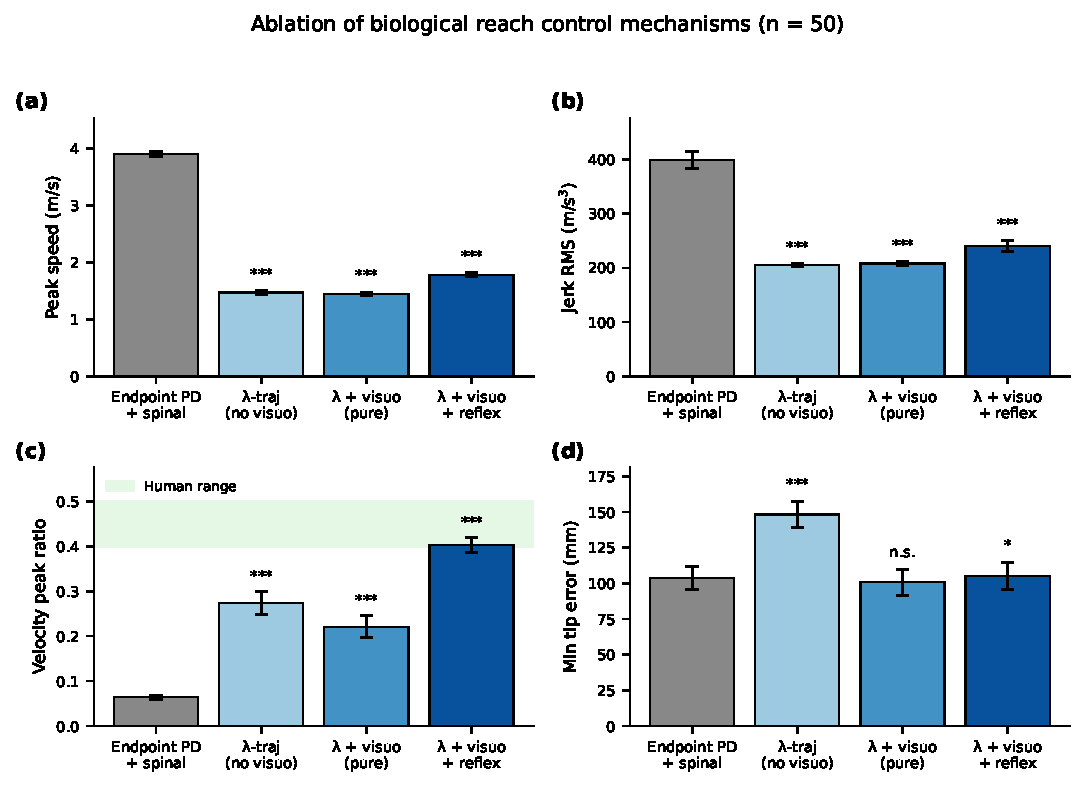
\includegraphics[width=\textwidth]{../../figures/fig1_ablation.pdf}
  \caption{\textbf{Ablation of biological reach control mechanisms.}
  \textit{Minimum-tip-error distributions overlap across all controllers
  (panel d), but only the biologically-grounded $\lambda$-EP variants
  partially reproduce the peak-timing and smoothness invariants of human
  reach.}
  \textbf{(a)} Peak tip speed. Endpoint-PD~+~spinal (gray) overshoots at
  $\approx 3.9$ m s$^{-1}$, whereas the static $\lambda$-trajectory
  baseline (light blue) and the $\lambda$~+~visuomotor controller with
  reflexes (dark blue) remain within $\approx 1.5$--$1.8$ m s$^{-1}$,
  matching reported human values for $\sim 50$ cm reaches \citep{morasso1981}.
  \textbf{(b)} Root-mean-square jerk. Reflexes do not increase smoothness
  costs.
  \textbf{(c)} Velocity-peak ratio (vpr): the time of peak speed
  normalised by movement duration. Only the +reflex controller falls
  inside the human band ($0.40$--$0.50$, green).
  \textbf{(d)} Minimum tip-error. The endpoint-PD~+~spinal, pure
  $\lambda$~+~visuomotor, and +reflex headline conditions cluster near
  $\approx 100$ mm and remain within the pre-defined $\pm 20$ mm
  practical equivalence margin (\S2.7, \S3.1); the no-visuomotor
  $\lambda$-trajectory condition reaches less accurately ($\approx 148$
  mm), consistent with \S3.2 where visuomotor feedback is identified as
  the primary accuracy component.
  Bars show mean~$\pm$~SEM ($n = 50$ randomised seeds per condition).
  Significance is reported relative to the endpoint-PD~+~spinal baseline
  (\S2.6) by the seed-paired Wilcoxon signed-rank test ($^{*}p<0.05$,
  $^{**}p<0.01$, $^{***}p<0.001$; n.s.~$=$~not significant), in line
  with the paired seed design described in \S2.7.}
  \label{fig:1}
\end{figure}

\begin{figure}[h]
  \centering
  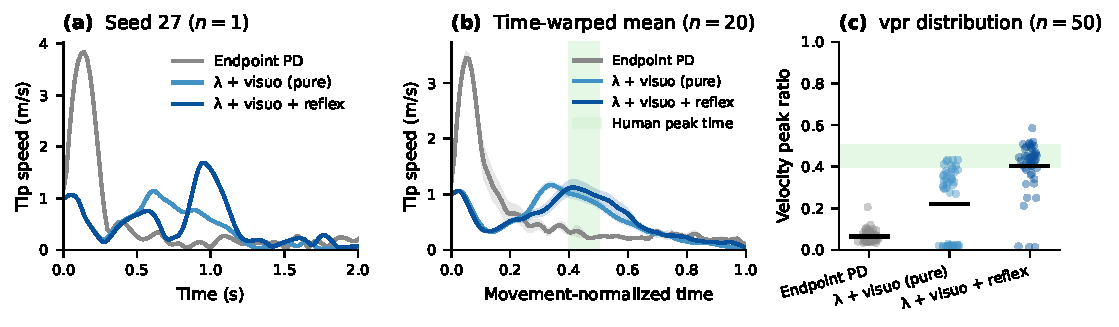
\includegraphics[width=\textwidth]{../../figures/fig2_velocity_profiles.pdf}
  \caption{\textbf{Velocity profiles.}
  \textit{Adding spinal reflexes to the $\lambda$-EP controller transforms
  a multi-peak speed profile into a single dominant profile whose peak
  timing falls inside the human reference band.}
  \textbf{(a)} Tip-speed profiles for a single representative seed (seed
  27, $n = 1$). The endpoint-PD~+~spinal baseline (gray) produces an
  initial ballistic spike followed by oscillatory residuals. The pure
  $\lambda$~+~visuomotor controller (light blue) shows two prolonged
  peaks. Adding stretch reflexes (dark blue) yields a single dominant
  peak near $1.7$ m s$^{-1}$ with peak timing inside the human band; the
  profile retains a small initial transient and a residual right-skewness
  (see \S3.1).
  \textbf{(b)} Time-warped mean speed across $n = 20$ seeds (the ablation
  seed list of \S3.2; movement window defined by speed $> 0.02$
  m s$^{-1}$). Shaded band $=\pm 1$ SEM. Green band marks the human
  peak-time range ($0.40$--$0.50$ of normalised movement time). The
  +reflex condition (dark blue) is the only one whose mean profile peaks
  inside this band.
  \textbf{(c)} Per-seed velocity-peak ratio across the headline $n = 50$
  seeds of \S3.1. Black bars $=$ mean. Green band $=$ human reference
  range \citep{morasso1981, flashhogan1985}. The change of $n$ between
  panels (b) and (c) is intentional: panel (b) shares the $n = 20$ seed
  list with the ablation analysis (Fig.~\ref{fig:4}), and panel (c)
  reports the headline $n = 50$ distribution.}
  \label{fig:2}
\end{figure}

\begin{figure}[h]
  \centering
  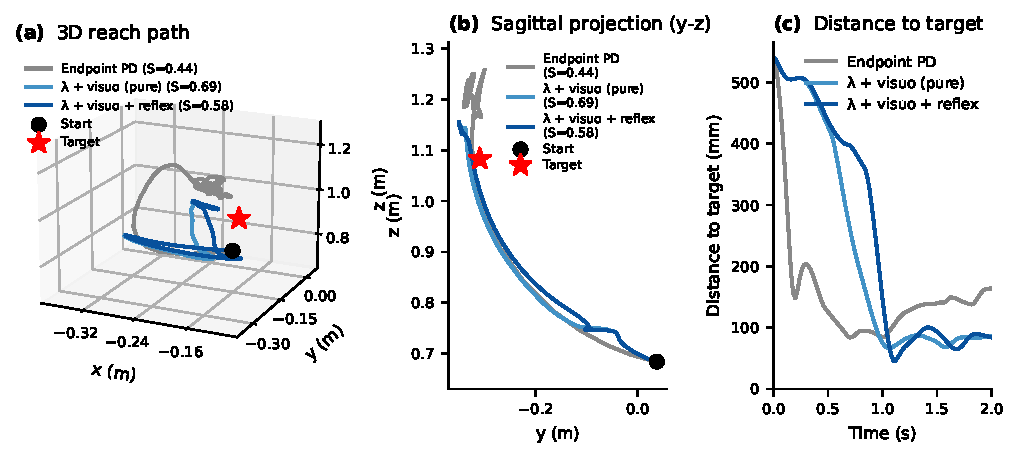
\includegraphics[width=\textwidth]{../../figures/fig3_trajectories.pdf}
  \caption{\textbf{End-effector trajectories.}
  \textit{The $\lambda$-EP controller produces straighter and more direct
  end-effector paths than the engineering baseline.}
  \textbf{(a)} 3-D reach paths for a representative seed (seed 27). Black
  circle $=$ start, red star $=$ target. The straightness ratio $S$
  (straight-line distance / path length, higher $=$ straighter) is shown
  in each legend entry.
  \textbf{(b)} Sagittal projection ($y$--$z$ plane) of the same
  trajectories, illustrating the qualitative difference between the
  early ballistic overshoot of endpoint-PD and the smoother arc of the
  $\lambda$-EP controllers.
  \textbf{(c)} Distance-to-target time courses. The $\lambda$-EP
  controllers approach the target monotonically; endpoint-PD oscillates
  around the residual $\approx 100$ mm offset throughout the 2 s
  movement window.}
  \label{fig:3}
\end{figure}

\begin{figure}[h]
  \centering
  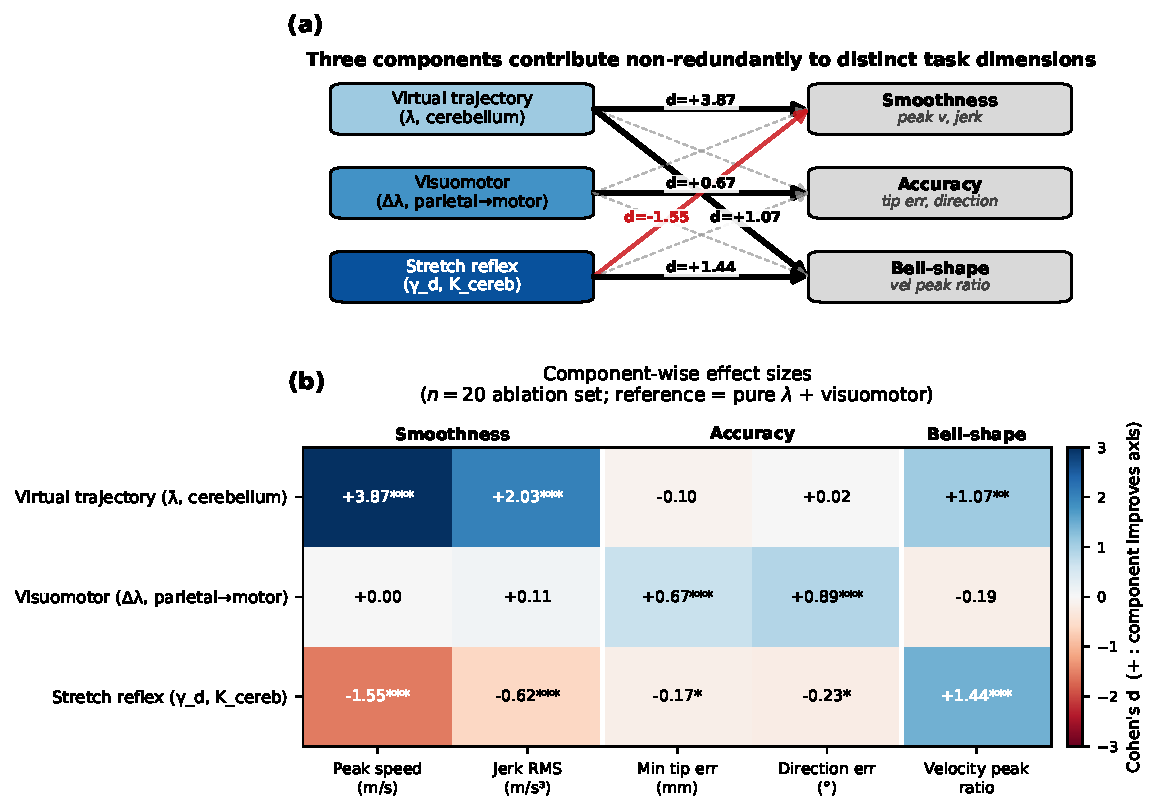
\includegraphics[width=\textwidth]{../../figures/fig4_orthogonal.pdf}
  \caption{\textbf{Component contributions of the three controller
  layers.}
  \textit{Each controller component contributes preferentially to one
  task dimension (smoothness, accuracy, or velocity-peak timing), with
  two practically-sized off-diagonal effects.}
  \textbf{Reference configuration is the pure $\lambda$~+~visuomotor
  controller (no reflexes, no cerebellar correction), not the
  endpoint-PD~+~spinal baseline of \S3.1; signed Cohen's $d$ is reported
  with the convention positive $=$ improvement (lower for error / peak
  speed / jerk; higher for vpr).}
  \textbf{(a)} Component-to-axis schematic. Three components --- virtual
  trajectory ($\dot{\boldsymbol{\lambda}}$, light blue), visuomotor
  feedback ($\Delta\boldsymbol{\lambda}$, mid blue), and the spinal
  reflex layer (dark blue; the optional cerebellar correction is treated
  separately in \S3.3 and is not part of this ablation) --- project onto
  three behavioural axes (smoothness, accuracy, velocity-peak timing).
  Black solid arrows mark improvements with $|d| > 0.5$ (signed Cohen's
  $d$ based on the primary metric for each axis: peak speed, minimum
  tip error, and velocity-peak ratio respectively); red arrows mark
  degradations of equivalent magnitude; thin dashed gray arrows mark
  weak effects ($|d| \le 0.5$).
  \textbf{(b)} Signed Cohen's $d$ for each component~$\times$~metric
  pair ($n = 20$ seeds per condition; data from the F13 ablation).
  Positive values (blue) indicate that adding the component pushes the
  metric in the behaviourally desirable direction (lower for error /
  speed / jerk; higher for vpr). Asterisks denote the seed-paired
  Wilcoxon signed-rank test ($^{*}p<0.05$, $^{**}p<0.01$,
  $^{***}p<0.001$); Cohen's $d$ is shown as the distribution-level
  effect size. The block-diagonal pattern demonstrates that the three
  components contribute non-redundantly, with two practically-sized
  off-diagonal terms --- virtual trajectory has a secondary positive
  effect on bell shape ($d = +1.07^{**}$) and reflexes have a moderate
  negative effect on peak-speed control ($d = -1.55^{***}$) --- and two
  small but paired-significant accuracy costs of reflexes
  ($d = -0.17^{*}$ on minimum tip error, $d = -0.23^{*}$ on direction
  error).}
  \label{fig:4}
\end{figure}

\begin{figure}[h]
  \centering
  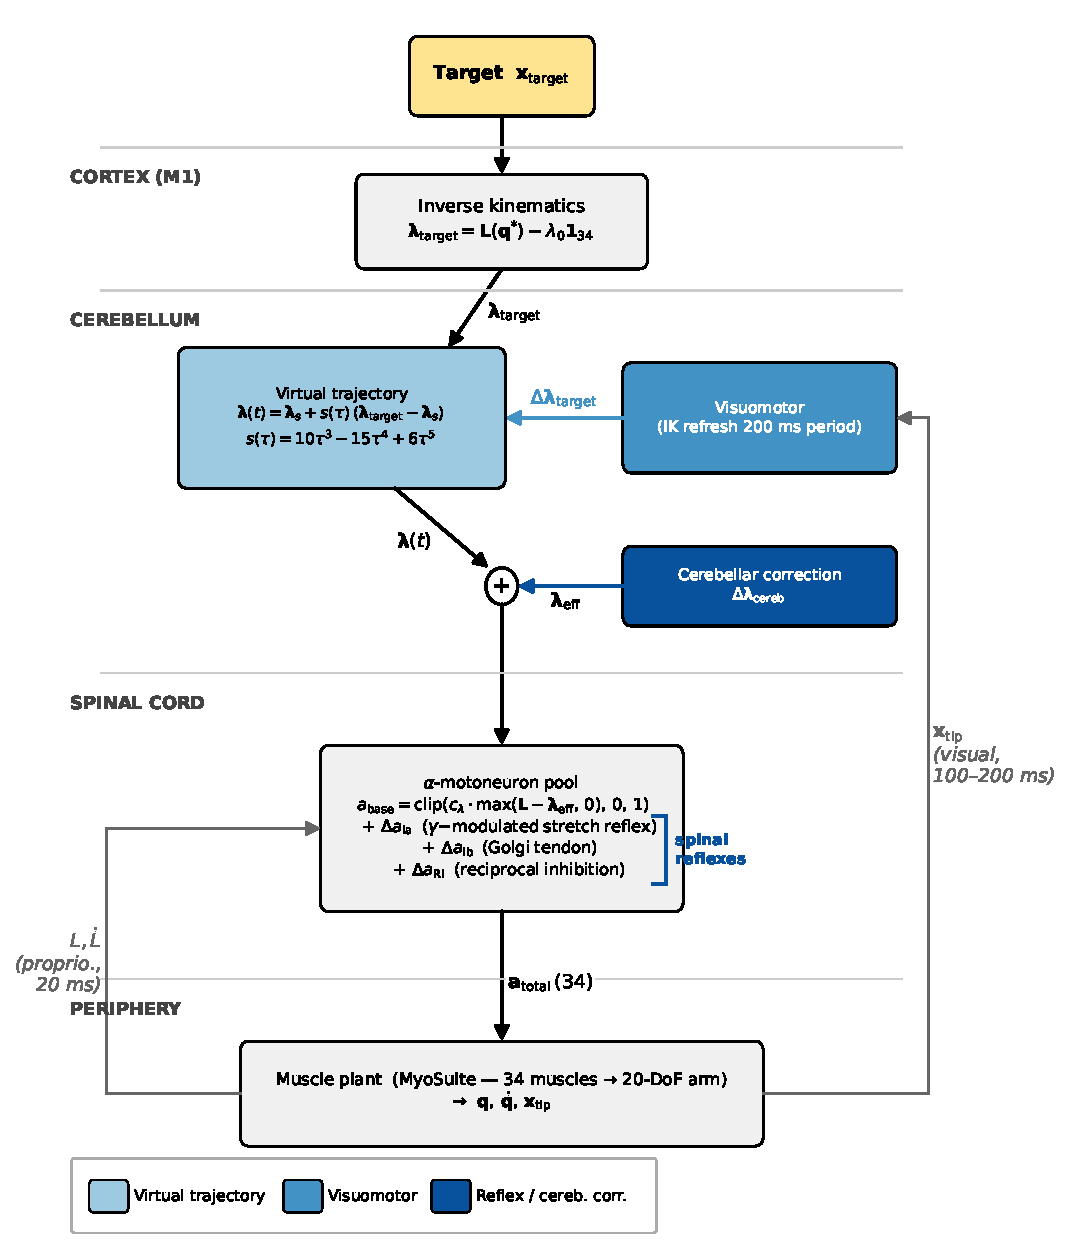
\includegraphics[width=\textwidth]{../../figures/fig5_architecture.pdf}
  \caption{\textbf{Controller architecture.}
  \textit{Block diagram of the neuromusculoskeletal reach controller,
  organised by anatomical level. Cortical, cerebellar and spinal blocks
  are kept distinct; the figure is a functional schematic, not a strict
  neuroanatomical mapping.}
  A target position $\mathbf{x}_{\mathrm{target}}$ provided by the visual
  system (top) drives an inverse-kinematics solver at the
  \textbf{cortical/planning} level that returns the equilibrium muscle
  thresholds
  $\boldsymbol{\lambda}_{\mathrm{target}} = \mathbf{L}(\mathbf{q}^{*}) -
  \lambda_{0}\mathbf{1}_{34}$
  and generates a minimum-jerk virtual trajectory
  $\boldsymbol{\lambda}(t) = \boldsymbol{\lambda}_{s} +
  s(\tau)(\boldsymbol{\lambda}_{\mathrm{target}}-\boldsymbol{\lambda}_{s})$,
  $s(\tau) = 10\tau^{3}-15\tau^{4}+6\tau^{5}$ \citep{flashhogan1985}.
  A separate \textbf{parietal--motor visuomotor block} updates
  $\boldsymbol{\lambda}_{\mathrm{target}}$ from the observed tip
  position every 200 ms, and an \emph{optional} \textbf{cerebellar
  branch} (dashed in the figure) adds a predictive correction
  $\Delta\boldsymbol{\lambda}_{\mathrm{cereb}}$ from a CfC forward-model
  prediction error (this branch is the negative-result configuration of
  \S2.5 and \S3.3 --- disabled in the headline controller). The
  resulting effective threshold
  $\boldsymbol{\lambda}_{\mathrm{eff}}$ projects to the \textbf{spinal}
  $\alpha$-motoneuron pool, where a base activation
  $\mathbf{a}_{\mathrm{base}} =
  \mathrm{clip}(c_{\lambda}\cdot\max(\mathbf{L}-
  \boldsymbol{\lambda}_{\mathrm{eff}},0),0,1)$
  is augmented by an Ia stretch reflex
  $\Delta\mathbf{a}_{\mathrm{Ia}}$ ($\gamma$-MN-modulation slot retained
  but disabled, see \S2.4), a Golgi-tendon component
  $\Delta\mathbf{a}_{\mathrm{Ib}}$, and reciprocal inhibition
  $\Delta\mathbf{a}_{\mathrm{RI}}$.
  The summed activation $\mathbf{a}_{\mathrm{total}}$ drives the
  MyoSuite myoArm muscle plant (34 muscles, 20-DoF arm), whose output
  state $(\mathbf{q}, \dot{\mathbf{q}}, \mathbf{x}_{\mathrm{tip}})$
  feeds back to the spinal pool with a 20 ms proprioceptive delay
  (left loop) and to the visuomotor block with a 100--200 ms visual
  delay (right loop). Component colours match those used in
  Figs.~\ref{fig:1}--\ref{fig:4}.}
  \label{fig:5}
\end{figure}

\backmatter

\section*{Declarations}

\paragraph{Funding.} The author declares that no external funding was received for this work.

\paragraph{Competing interests.} The author declares that he has no competing interests.

\paragraph{Author contributions.} This is a single-author work. JK conceived the study, designed and implemented the controllers and the evaluation pipeline, performed the experiments and analyses, prepared the figures, and wrote the manuscript.

\paragraph{Ethics approval.} Not applicable. This study used only computational simulations and did not involve human participants, animals, or biological samples.

\paragraph{Consent to participate / Consent for publication.} Not applicable.

\paragraph{Availability of data and materials.} The complete implementation, exact seed lists, raw per-seed metric tables, trained CfC weights, and figure-generation pipeline are released under the MIT license at the GitHub repository \href{https://github.com/jkoba0512/myoarm-lambda-ep}{\texttt{jkoba0512/myoarm-lambda-ep}} and archived as Zenodo \href{https://doi.org/10.5281/zenodo.19948021}{10.5281/zenodo.19948021} (release \texttt{v1.0.0-bioRxiv}). The reproduction commands are documented in the repository \texttt{README}. The seed-reproducibility helper (\texttt{deterministic\_reset}) for the MyoSuite reach environments is provided in \texttt{src/myoarm/env\_utils.py}.

\paragraph{Code availability.} See ``Availability of data and materials'' above. All code is included in the same release.

\paragraph{Preprint.} A preprint of this manuscript has been posted on bioRxiv: \href{https://doi.org/10.64898/2026.05.01.722167}{10.64898/2026.05.01.722167} (2026-05-06).

%%========================================================================%%
%% References - natbib + SPBASIC style. Source bibliography database is   %%
%% paper/tex/references.bib. Bibliography keys correspond to those used   %%
%% in \citet / \citep / \citealt commands throughout the body.            %%
%%========================================================================%%

%% Note: sn-jnl.cls already issues \bibliographystyle{sn-basic} when the
%% [sn-basic] option is given on \documentclass, so we do NOT repeat it
%% here (would trigger 'Illegal, another \bibstyle command' in bibtex).
\bibliography{references}

\end{document}
